\begin{abstract}
The bad patch finder of Will Stevens' scrollreading chain discards pieces of surface that cannot sit together, and on three tangled growths of PHerc.~1447 it ran for hours and was abandoned. We made two changes inside its one function. The first stops the enumeration from extending a chain that is already dead, and the second replaces a map rebuilt on every pass with a vector. On a quiet machine the \texttt{c} stage of the tangle seed40 goes from \BenchPlainSeedFortyMax{} s to \BenchBothSeedFortyMedian{}, about two hundred times faster. On seed38 it goes from \BenchPlainSeedThirtyEightMax{} s to \BenchBothSeedThirtyEightMedian{}, a factor that a disturbance of the untouched run can only have inflated. On a ribbon, where the enumeration was never the cost, the factor is only \BothChangesFactor{}. Every file the five delivery stages write is byte identical between the arms on fifteen named growth trees of two scrolls, and the stage's whole standard output is identical on fourteen of them. A third change, a guard, turns an abort into a result on a tree whose alignment file names missing patches. The changes make a search over many seeds affordable but move no delivered square. The main limit is that identity is not correctness.
\end{abstract}
The organisers of the Vesuvius Challenge ask how to make the reading of a scroll work ``automatically, reliably, and at scale for every scroll''~\cite{openproblems2026}. Will Stevens' program has a step that finds the pieces of surface that cannot sit together and throws them away. On three tangled growths of PHerc.~1447 that step ran for hours and was abandoned before a single sheet came out. Measured against his program as published, on two scrolls, PHerc.~1447 and PHerc.~0139, our changes make it finish quickly and leave every file it writes identical. Fig.~\ref{fig:s7} shows where those abandoned tangles lay: in the air around the scroll, while on the seeds that grew on the papyrus the step was never the slow one. A step that finishes on every tree is what lets the chain run over a whole scroll with nobody watching it, and whoever reads a scroll needs whole sheets before there is anything to read.

\begin{figure*}[t]
\centering
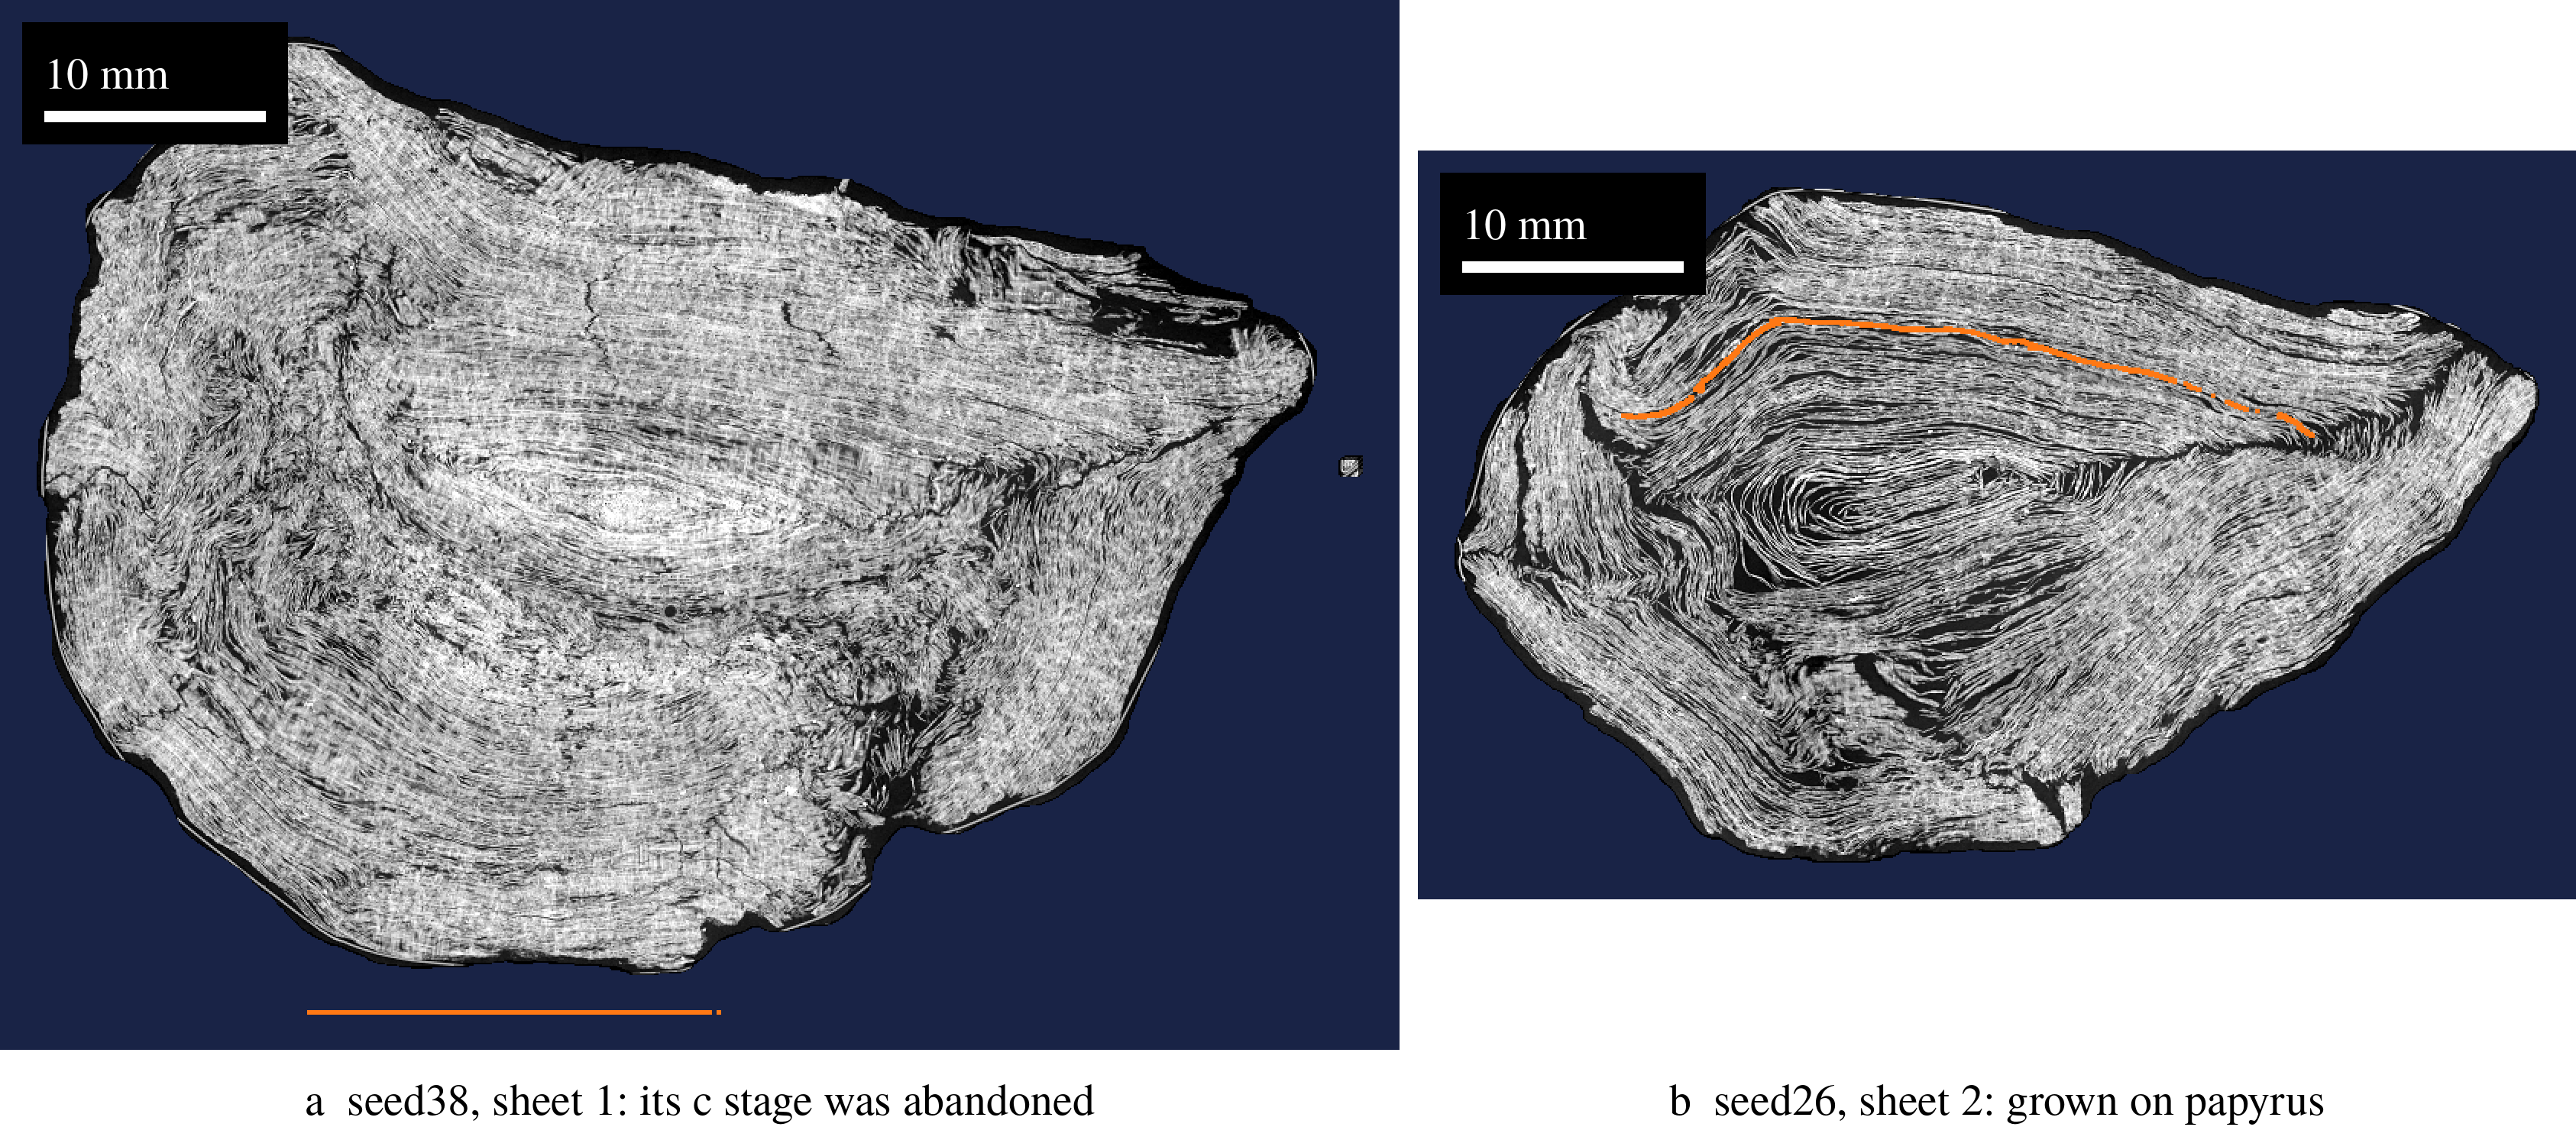
\includegraphics[width=0.9\textwidth]{figures/s-f7-a-sheet-the-old-stage-abandoned}
\caption{\textbf{A sheet the old stage abandoned, on the scroll it was grown in.} Each panel is one horizontal slice of the scan of PHerc.~1447, seen from above. Papyrus is grey, and dark blue is outside the scan's mask, where there is no scroll. Orange is where a delivered sheet crosses the slice. Panel a is the largest sheet of the trees whose untouched bad patch finder the seed runner stopped, seed38's sheet 1: it is a straight wall in the air beside the scroll. Panel b, for comparison, is the largest sheet of the seeds that grew on papyrus, seed26's sheet 2, which follows a turn of the papyrus. The white bar is 10 mm.}
\label{fig:s7}
\end{figure*}

Our contribution is two changes to that step, S1 and S2, with the evidence that they change no byte the chain writes. We add a guard, S3, that lets the step finish on a tree where it aborted. The program, its stages and the growth that feeds them are Stevens'~\cite{stevensrepo}. The arm we compare against already carries an earlier performance series of this project, which section 4 remeasures. The assembly of this chain on PHerc.~0826 is measured in a separate article sent with this one~\cite{pherc0826chain}.

\section*{What this work is about, in plain words}

The scrolls from Herculaneum were burnt by a volcano. They cannot be unrolled by hand, so they are scanned, and software has to find the sheets of papyrus inside the scan. Each sheet is then flattened so the writing on it can be read.

This work is about one program in that chain, written by Will Stevens~\cite{stevensrepo}. The program first grows many small pieces of surface, called patches. A later step looks for patches that cannot be joined to their neighbours consistently, and throws those away.

On three of the growths that step did not finish, and our runner stopped it at its time limit. Two changes inside it make the same step finish in about a minute. Nothing it produces changes: every file the chain writes afterwards is identical, byte for byte, to the file it wrote before.

A third change repairs a crash. On one growth the program stopped with an error because its own bookkeeping named pieces that were not on disk. It now refuses those pieces and says how many it refused, instead of stopping.

A reader can check all of this. Every number in this work points to the file it was read from, through a marker and the appendix, and every one of those files is in this folder. The claim that nothing changed is a comparison of every file the chain writes, not of the finished pictures alone. Where a measurement was taken on a busy machine, the text says so.

\section{The chain and its stages, on two scrolls}

This section introduces the chain, the three changes and the two scrolls, and shows that once the changes are in, the \texttt{c} stage is no longer the whole cost of a run.

The object is the patch based surface tracing chain of Will Stevens~\cite{stevensrepo}, \protect\path{pipeline9/simpaper10} of the scrollreading repository at commit \texttt{62cbc21}, which is \protect\path{refs/heads/main} of the clone on this disk {\prov{1}}. The copy of \protect\path{simpaper10.cpp} the builds here were laid from hashes to the same blob as \protect\path{62cbc21:pipeline9/simpaper10.cpp}. A run is a growth, \texttt{g 36000}, followed by five delivery stages: \texttt{c}, \texttt{l}, \texttt{vm 10}, \texttt{hm 10}, \texttt{fm 30 10}. The growth writes patches and an alignment file, \protect\path{rel.csv}, one line per alignment between two patch numbers. The \texttt{c} stage, the bad patch finder, reads them both, enumerates chains of patches of length 2 to 5, scores them, and condemns the patches that cannot be placed consistently.

\subsection{The three changes this work proposes, and how they are named here}

The series these patches belong to numbers them on disk, and those numbers mean nothing to a reader. This work calls them S1, S2 and S3, in the order the text meets them, and the serial appears only in the last column.

\begin{table*}[t]
\centering
\small
\begin{tabularx}{\textwidth}{XXXXXX}
\toprule
 & what it is & what it does & measured effect & identity & on disk \\
\midrule
S1 & a dead prefix is not extended & when a chain dies the odometer advances at the position it died, instead of enumerating every suffix of a prefix already rejected & with S2, the \texttt{c} stage of the tangle seed40 goes from \BenchPlainSeedFortyMax{} s to \BenchBothSeedFortyMedian{}, \QuietFactorSeedFortyMedian{} times, and of seed38 from \BenchPlainSeedThirtyEightMax{} to \BenchBothSeedThirtyEightMedian{} & every file the five stages write, byte for byte, on fifteen named trees & \protect\path{corrections/00008} \\
S2 & the cover's frequency table is a vector & the greedy cover rebuilt a \texttt{std:\allowbreak{}:\allowbreak{}map} of counts on every pass; patch numbers are small integers, so one cleared vector holds the same counts & measured with S1 above; on a ribbon the pair is \BothChangesFactor{} times, which the work states rather than averages away & the same & \protect\path{corrections/00009} \\
S3 & a chain through a patch with no geometry is refused & the alignment map has keys the patches map does not; the stage aborted on the first such chain, and the guard counts and refuses it at the point the chain is assembled & turns an abort into a run on the one tree where it happens, and costs time on three of the seven ribbons of the reference scroll & byte identical on the three trees with no such patch & \protect\path{corrections/00007} \\
\emph{the earlier performance patch} & the selection render state is cleared per touched cell and the normals are precomputed & it is not one of the three and is listed here because this work remeasures it: its own study no longer exists & \EarlierPatchFactorMedian{} times on the ribbon of \SeedPatchesTwentySix{} patches, median against median & the whole downstream on fresh copies of two growth trees, one of each scroll: \EarlierPatchFilesCompared{} files compared, none differing, and the only difference in anything either arm prints is one line, \texttt{points skipped as off-\allowbreak{}grid:\allowbreak{} 0}, which only the arm with the patch writes & \protect\path{performance/00002} \\
\bottomrule
\end{tabularx}
\end{table*}

The prose below says S1, S2 and S3. The earlier performance patch is in the table because this work remeasures both of the things it claims, its factor and its identity. Neither could be read back from anything on this disk when the work was begun. It is not one of the three, and the prose never counts it among them. Its identity was measured on 2026-09-22, file by file and on the printed output {\prov{2}}.

All three changes are now on the author's repository, where they were opened on 22 September 2026. S1, S2 and S3 are one pull request, WillStevens/scrollreading \#4, which is stacked on \#3: that one carries the earlier performance patch alone, because the three do not apply to \texttt{main} without it. The defect behind the crash of section 5, a growth started into a folder that already holds one, is issue \#2 on the same repository.

Two scrolls are used, and they are not interchangeable. The voxel of PHerc. 1447 is 8.640 um, the scroll's own value from the dataset manifest {\prov{68}}. PHerc. 0139, whose voxel is \VoxelZeroOneThreeNine{} um, is used here only as a second body of growth trees on which byte equality and stage times can be checked.

The next table gives what the five stages cost on the arm carrying the two changes of section 4, at four OpenMP threads {\prov{69}}. Only the \texttt{c} row was timed on a quiet machine. The other four were timed on a machine shared with other studies, with 7.2 to 8.4 of its 24 cores busy.

\begin{table*}[t]
\centering
\small
\begin{tabularx}{\textwidth}{XXXX}
\toprule
stage & seed26, a ribbon, \SeedPatchesTwentySix{} patches & seed40, a tangle, \SeedPatchesForty{} patches & machine \\
\midrule
\texttt{c} & \BenchBothSeedTwentySixMedian{} & \BenchBothSeedFortyMedian{} & quiet, 0.05 to 0.12 cores busy of 24 \\
\texttt{l} & 2.5 & 5.3 & shared, \StageLoadLow{} to \StageLoadHigh{} \\
\texttt{vm 10} & 2.5 & 5.4 & shared, \StageLoadLow{} to \StageLoadHigh{} \\
\texttt{hm 10} & 0.1 & 0.1 & shared, \StageLoadLow{} to \StageLoadHigh{} \\
\texttt{fm 30 10} & \StageFmSecondsSeedTwentySix{} & 6.2 & shared, \StageLoadLow{} to \StageLoadHigh{} \\
\bottomrule
\end{tabularx}
\end{table*}

The \texttt{c} row is the median of three runs on a machine doing nothing else {\prov{3}}. On the ribbon the three runs took \BenchBothSeedTwentySixMin{}, \BenchBothSeedTwentySixMedian{} and \BenchBothSeedTwentySixMax{} s. On the tangle they took \BenchBothSeedFortyMin{}, \BenchBothSeedFortyMedian{} and \BenchBothSeedFortyMax{} s. Their spreads are 2.53 and 3.19 per cent of the smallest run {\prov{21}}. The four rows below the \texttt{c} row are single timings from the earlier harness on a shared machine and have not been repeated quietly. The column therefore mixes two kinds of measurement, and the table says which is which rather than presenting five numbers of equal weight.

What matters in this table is the proportion. The four stages after \texttt{c} cost 17.0 seconds on the tangle and 18.9 on the ribbon, summed from the same file. Before the changes, the \texttt{c} stage of that same tangle took \BenchPlainSeedFortyMax{} s on the quiet bench {\prov{21}}, so it was not one stage among five: it was the run. The growth that precedes them takes 2,400 to 10,075 s over the nine trees of section 2 {\prov{5}}. Those growths ran two or three at a time beside each other, which makes their wall clocks a cost record and not a result.

\section{Ten drawn seeds on PHerc. 1447}

This section shows that the growth trees of PHerc. 1447 fall into two kinds, ribbons and tangles. The kind predicts the cost of the \texttt{c} stage but not the size of the sheet the chain delivers.

Ten seed points were drawn on PHerc. 1447 and grown {\prov{6}}. Nine of the ten finished their growth by themselves and were delivered and measured. seed11's growth returned 3, so it is counted apart in every column and never folded into a median with the others.

The fan out of a tree is the average number of neighbours a patch has in its alignment map. It splits the ten trees into two groups with nothing in between. Ribbons grew as one long strip and are cheap for the \texttt{c} stage. Tangles grew folded on themselves and are expensive. \texttt{AugmentAlignmentMap} inserts the reverse of every alignment, so the map the chain walk sees is symmetric, and its mean fan out is twice the edge count over the number of keys {\prov{7}}.

\begin{table*}[t]
\centering
\small
\begin{tabularx}{\textwidth}{XXX}
\toprule
kind & seeds & fan out \\
\midrule
ribbon & seed26, seed01, seed15 & \FanOutSeedTwentySix{}, \FanOutSeedOne{}, \FanOutSeedFifteen{} \\
tangle & seed38, seed40, seed48, seed44, seed11, seed34, seed35 & \FanOutSeedThirtyEight{}, \FanOutSeedForty{}, \FanOutSeedFortyEight{}, \FanOutSeedFortyFour{}, \FanOutSeedEleven{}, \FanOutSeedThirtyFour{}, \FanOutSeedThirtyFive{} \\
\bottomrule
\end{tabularx}
\end{table*}

One prediction was written before its answer existed, and it was right. The kind of a tree can be read from the growth's own log long before the growth ends, and seed44 is the one seed where that rule was applied in advance rather than fitted. The reading was taken 532 seconds into a growth that then ran 9,097 s. By then the share of the first 100,000 log lines stood at 0.11963, against a ribbon band that topped out at 0.04275. The prediction recorded was tangle. Its note said that the share sat in the gap between the two bands, 0.00039 below the nearest tangle rather than inside the tangle band {\prov{8}}. The answer row, appended when the growth ended, reads tangle at fan out \FanOutSeedFortyFour{}. The rule has since gained a repeat control it did not have when it was written. The same seed was grown twice, under different machine states, to logs of 4,010,300 and 3,348,977 lines. The two shares differ by 0.00005, against a gap of about 0.07 between the kinds {\prov{9}}.

The measure of a delivered sheet used throughout is its square: the side of the exact largest axis aligned, fully covered square in the sheet, at that scroll's own voxel. Over the three seeds on papyrus, the largest square is \SeedSquareTwentySix{} mm, on seed26, and the smallest is \SeedSquareOne{} mm, on seed01. The median is \SeedSquareFifteen{} mm, on seed15 {\prov{71}}. Those three seeds hand back thirty delivered sheets, ten per seed, and none of them reaches 20 mm {\prov{72}}. The other seven seeds, seed11, seed34, seed35, seed38, seed40, seed44 and seed48, are the seven tangles above, and they grew in air: the raw masked scan is absent at each of their seed points {\prov{73}}.

The fan out does not bound the square, and seed44 is the case that shows it. Nine seeds have both a fan out and a square. The three ribbons hold three of the four largest squares, \SeedSquareTwentySix{}, \SeedSquareFifteen{} and \SeedSquareOne{} mm. Five of the six tangles are at or below \SeedSquareThirtyEight{} {\prov{10}}. The sixth tangle is the counterexample, and it is the very seed the rule was applied to in advance. seed44, a tangle at fan out \FanOutSeedFortyFour{}, delivers \SeedSquareFortyFour{} mm, the third largest square of the nine. That is above the ribbon of seed01, at \SeedSquareOne{}, and below the other two ribbons.

A bound had been registered before seed44's downstream ran: a seed at or above fan out \FanOutSeedThirtyEight{} gives a square at or below \SeedSquareThirtyEight{} mm. The file called it ``likely, and it is the sixth test of a bound that is five for five'' {\prov{11}}. The delivered square is above it. The study recorded its own refutation in that file on 2026-09-22T02:23:46Z, as a second row appended beside the prediction rather than as an edit of it, because a preregistration is not rewritten. The prediction row's \texttt{answer} column still reads ``not yet known, the downstream has not been run'', which is what it said when it was written. The appended row's \texttt{answer} reads ``WRONG on both''. The square came out at \SeedSquareFortyFour{} mm against a bound of \SeedSquareThirtyEight{}. The traced area came out at \SeedTracedAreaFortyFour{} mm2 against a bound of 1,898.5. The fan out, in short, orders the cost of the \texttt{c} stage sharply, which is the subject of section 3, and it does not bound the square.

\section{Where the c stage's time goes}

This section shows where the untouched \texttt{c} stage spends its time: in the descent of a \texttt{std:\allowbreak{}:\allowbreak{}map}, driven by an enumeration whose size grows with the fourth power of the fan out.

A profile was taken before anything was changed, with \texttt{perf record -\allowbreak{}F 299 -\allowbreak{}e cycles:\allowbreak{}u}, over the first \ProfileBaselineSeconds{} s of the untouched stage on a fresh copy of seed40's tree. The run was stopped by a signal at that point, and its return code reads -15 {\prov{12}}. The profile file carries the shares and not the duration. The binary carried \texttt{-\allowbreak{}g} and nothing else: its \texttt{.\allowbreak{}text} section is byte for byte that of the same build without \texttt{-\allowbreak{}g} {\prov{13}}, so the profile is of the code that ships.

\begin{table*}[t]
\centering
\small
\begin{tabularx}{\textwidth}{XXX}
\toprule
share & what & sort \\
\midrule
\ProfileShareFindBadPatches{} \% & \texttt{BadPatchFinder:\allowbreak{}:\allowbreak{}FindBadPatchesGeneral} & symbol \\
\ProfileShareRightChild{} \% & \texttt{stl\_\allowbreak{}\allowbreak{}tree.\allowbreak{}h:\allowbreak{}1437}, the right child step of a red black descent & source line \\
\ProfileShareLowerBoundOne{}, \ProfileShareLowerBoundTwo{}, \ProfileShareLowerBoundThree{}, \ProfileShareLowerBoundFour{} \% & \texttt{stl\_\allowbreak{}\allowbreak{}tree.\allowbreak{}h:\allowbreak{}2604,\allowbreak{} 2605,\allowbreak{} 2603,\allowbreak{} 2607}, the body of \texttt{\_\allowbreak{}\allowbreak{}M\_\allowbreak{}\allowbreak{}lower\_\allowbreak{}\allowbreak{}bound} & source line \\
\ProfileShareLeftChild{} \% & \texttt{stl\_\allowbreak{}\allowbreak{}tree.\allowbreak{}h:\allowbreak{}1425}, the left child step & source line \\
\ProfileShareOdometerWalk{} \% & \texttt{badpatchfinder.\allowbreak{}cpp:\allowbreak{}426}, the odometer's rewalk of the chain & source line \\
\bottomrule
\end{tabularx}
\end{table*}

About eighty per cent of the stage, then, is the descent of a \texttt{std:\allowbreak{}:\allowbreak{}map}, and the line of the chain's own source that drives it is the odometer's validity walk.

To see why, it helps to count the work instead of timing it. The enumeration is an odometer over \texttt{indices[0.\allowbreak{}length-\allowbreak{}1]}, a counter that walks every run of patches in turn. The number of index tuples it visits for a chain of length L is the number of walks of L minus 1 edges in the augmented alignment multigraph. That count can be taken exactly from a tree's own \protect\path{rel.csv} and \protect\path{patches/}, with no run at all {\prov{14}}. A counting build of the stage itself, with one increment per visit of the \texttt{while} body, agrees with it to the step: on seed26 both read 10,761,063 over the four rounds {\prov{15}}. The count was taken this way because the untouched binary, given the same tree at four threads, had not begun the round at length 5 after 3,000 s {\prov{16}}.

\begin{table*}[t]
\centering
\small
\begin{tabularx}{\textwidth}{XXXXX}
\toprule
tree & length 2 & length 3 & length 4 & length 5 \\
\midrule
seed26, fan out \FanOutSeedTwentySix{} & \StepsModelSeedTwentySixLengthTwo{} & \StepsModelSeedTwentySixLengthThree{} & \StepsModelSeedTwentySixLengthFour{} & \StepsModelSeedTwentySixLengthFive{} \\
seed40, fan out \FanOutSeedForty{} & 460,985 & \StepsModelSeedFortyLengthThree{} & \StepsModelSeedFortyLengthFour{} & \StepsModelSeedFortyLengthFive{} \\
seed40 with S1 of section 4, counted & 460,985 & \StepsPrunedSeedFortyLengthThree{} & \StepsPrunedSeedFortyLengthFour{} & \StepsPrunedSeedFortyLengthFive{} \\
\bottomrule
\end{tabularx}
\end{table*}

seed40 totals \StepsModelTotalSeedForty{} steps, and the round at length 5 is \StepsShareLengthFiveSeedForty{} per cent of them {\prov{17}}. The walk grows with the fourth power of the fan out at the longest length the stage runs. The file of fan outs states that as a cost model of the walk in the source, not as a measured time {\prov{74}}. The exact counts above are the measurement, and the first two rows are the ones a reader should compare.

\section{Two changes and their proof}

This section describes the two changes, shows that they make the \texttt{c} stage finish on the tangles, and shows that every byte the chain writes stays the same.

Both are patch files of this project's series for that repository, applied after the orphan guard of section 5. Neither changes a decision the stage makes; both change how much work it does to reach the same decision.

The first change, S1, stops the enumeration from extending a prefix that is already dead. When the chain being built meets a repeated patch or a patch already condemned, the build loop breaks, but the odometer still advances its last index. Every suffix of a dead prefix is therefore enumerated one at a time, and rejected again for the reason the prefix was rejected for. The change records the position at which the chain died and advances the odometer there, resetting the indices below it to zero, which is where the carry would have left them. A bad first patch is the same argument at depth zero.

The second change, S2, makes the frequency table of the cover a vector. The greedy cover at the end of the same function condemns one patch per pass, and on every pass it rebuilds a \texttt{std:\allowbreak{}:\allowbreak{}map<int,\allowbreak{}int>\allowbreak{}} of counts from nothing. Patch numbers are small non-negative integers, so one vector indexed by patch number, cleared at the top of each pass, holds the same counts with no allocation and no tree descent. The scan order and the comparison are untouched, so the patch chosen on each pass is the same patch.

The build script laid down a working copy from the pinned upstream plus the series with both patches. It is byte for byte the working copy laid with the guard alone and then edited by the two change scripts {\prov{18}}. The patch files, and not a hand edited tree, are what was built and measured.

The first change shows in the step counts before it shows in any clock. On seed40 the counting build with S1 takes \StepsPrunedTotalSeedForty{} steps, against \StepsModelTotalSeedForty{} before {\prov{19}}. That is a factor of \StepsFactorSeedForty{} (Fig.~\ref{fig:s2}), and the last row of the table of section 3 gives the four rounds. On seed26 the two variants print the same number of kept chains at every length, which is the change's correctness read off the instrument itself. On the two shortest lengths those counts are 21,432 and 52,571. On the two longest they are 191,087 and 682,561. Neither number depends on the machine.

\begin{figure*}[t]
\centering
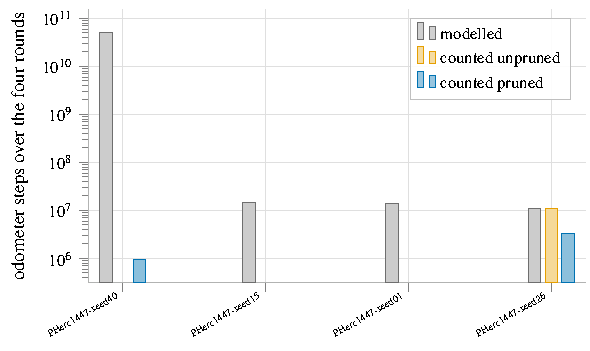
\includegraphics[scale=1]{figures/s-f2-odometer-steps}
\caption{\textbf{The odometer's steps, modelled against counted.} What the change does is not run faster, it is do less. On the tangle seed40 the enumeration as written takes \StepsModelTotalSeedForty{} steps and the changed one \StepsPrunedTotalSeedForty{}, a factor of \StepsFactorSeedForty{}, and that is a count of work and not a clock. The three ribbons sit three and a half orders of magnitude below the tangle before anything is changed. That is why the same change is worth about two hundred times on one and a factor of \BothChangesFactor{} on the other.}
\label{fig:s2}
\end{figure*}

With the enumeration pruned, the time moved elsewhere. A diagnostic build timed the three phases of the function with \texttt{omp\_\allowbreak{}\allowbreak{}get\_\allowbreak{}\allowbreak{}wtime} on seed40's tree {\prov{20}}.

\begin{table*}[t]
\centering
\small
\begin{tabularx}{\textwidth}{XXXXXX}
\toprule
arm & setup & odometer & sequences & cover & stage \\
\midrule
S3 and S1 & \TimersSetupSecondsCOne{} & \TimersOdometerSecondsCOne{} & \TimersSequencesSecondsCOne{} & \TimersCoverSecondsCOne{} & \TimersStageSecondsCOne{} s \\
S3, S1 and S2 & \TimersSetupSecondsCTwo{} & \TimersOdometerSecondsCTwo{} & \TimersSequencesSecondsCTwo{} & \TimersCoverSecondsCTwo{} & \TimersStageSecondsCTwo{} s \\
\bottomrule
\end{tabularx}
\end{table*}

After the first change the enumeration this work set out to fix costs \TimersOdometerSecondsCOne{} s, and the greedy cover costs \TimersCoverSecondsCOne{} s. That is why there is a second change, and why it is the one it is.

The next table gives the \texttt{c} stage on six seeds before the changes, with S1, and with both, at four threads for the arms {\prov{75}}. Both changed arms also carry the guard S3. Its times were taken on a shared machine, which is the weaker kind of measurement. The quiet bench has since retaken three of these seeds with nothing else running, and wherever a figure of this table is quoted elsewhere in this work, it is the quiet one.

\begin{table*}[t]
\centering
\small
\begin{tabularx}{\textwidth}{XXXXXX}
\toprule
seed & \protect\path{rel.csv} lines & before & S1 & S1 and S2 & note \\
\midrule
seed01 & \SeedRelLinesOne{} & 30 s & \CStageCOneSeedOne{} & \CStageCTwoSeedOne{} & before taken at 24 threads, not comparable \\
seed15 & \SeedRelLinesFifteen{} & 32 s & \CStageCOneSeedFifteen{} & \CStageCTwoSeedFifteen{} & before taken at 24 threads, not comparable \\
seed26 & \SeedRelLinesTwentySix{} & 22 s & \CStageCOneSeedTwentySix{} & \CStageCTwoSeedTwentySix{} & before taken at 24 threads, not comparable \\
seed38 & \SeedRelLinesThirtyEight{} & \CStageReferenceSeedThirtyEight{} s & \CStageCOneSeedThirtyEight{} & \CStageCTwoSeedThirtyEight{} & both arms on a shared machine \\
seed40 & \SeedRelLinesForty{} & 7,251 s & \CStageCOneSeedForty{} & 34.9 & both arms on a shared machine \\
seed48 & \SeedRelLinesFortyEight{} & \CStageReferenceSeedFortyEight{} s & \CStageCOneSeedFortyEight{} & \CStageCTwoSeedFortyEight{} & both arms on a shared machine \\
\bottomrule
\end{tabularx}
\end{table*}

Three of those rows have since been taken again on a machine that was doing nothing else, and the pair that matters most is one of them.

\begin{table*}[t]
\centering
\small
\begin{tabularx}{\textwidth}{XXXXX}
\toprule
tree & arm & runs & seconds & spread \\
\midrule
seed26, \SeedPatchesTwentySix{} patches & untouched & 2 & \BenchPlainSeedTwentySixMax{} and \BenchPlainSeedTwentySixMin{} & 2.4 s, 4.86 per cent of the smallest \\
seed26 & with both changes & 3 & \BenchBothSeedTwentySixMin{}, \BenchBothSeedTwentySixMax{}, \BenchBothSeedTwentySixMedian{} & 1.2 s, 2.53 per cent \\
seed40, \SeedPatchesForty{} patches & untouched & 1 & \BenchPlainSeedFortyMax{} & not measurable, one run \\
seed40 & with both changes & 3 & \BenchBothSeedFortyMax{}, \BenchBothSeedFortyMedian{}, \BenchBothSeedFortyMin{} & 1.1 s, 3.19 per cent \\
seed38, \SeedPatchesThirtyEight{} patches & untouched & 1 & \BenchPlainSeedThirtyEightMax{} & not measurable, one run \\
seed38 & with both changes & 3 & \BenchBothSeedThirtyEightMax{}, \BenchBothSeedThirtyEightMedian{}, \BenchBothSeedThirtyEightMin{} & \BenchBothSeedThirtyEightSpread{} s, \BenchBothSeedThirtyEightSpreadPct{} per cent \\
\bottomrule
\end{tabularx}
\end{table*}

Every run in that table used four threads, one run at a time, with 0.05 to 0.14 cores busy of 24 before each {\prov{21}}. On seed40 the quiet pair is \BenchPlainSeedFortyMax{} seconds against \BenchBothSeedFortyMedian{}, about two hundred times (Fig.~\ref{fig:s1}). The factor is \QuietFactorSeedFortyMedian{} taking the median of each arm, which is the shape every other factor in this work uses, and \QuietFactorSeedFortySmallest{} taking the smallest of each {\prov{22}}. On seed38 the quiet pair is \BenchPlainSeedThirtyEightMax{} seconds against \BenchBothSeedThirtyEightMedian{}, a factor of \QuietFactorSeedThirtyEightMedian{}, which the next paragraph qualifies. The shared machine's ratio on seed38 is \SharedRatioSeedThirtyEight{}, and on seed48, which the quiet bench did not retake, it is \SharedRatioSeedFortyEight{} {\prov{75}}.

\begin{figure*}[t]
\centering
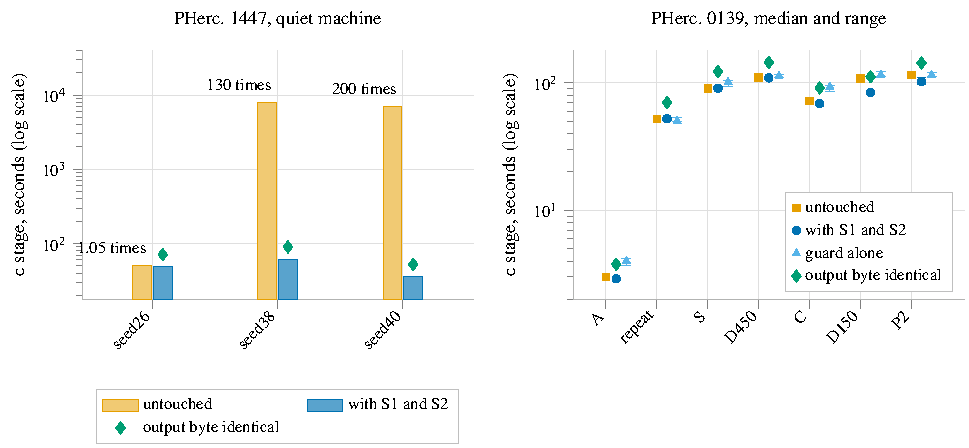
\includegraphics[scale=1]{figures/s-f1-c-stage-before-after}
\caption{\textbf{The \texttt{c} stage, untouched against changed, on the quiet bench.} On PHerc. 1447 the change is the difference between a stage that finishes and one that is abandoned. The untouched binary takes \BenchPlainSeedFortyMax{} s on one tangle and \BenchPlainSeedThirtyEightMax{} on the other. The changed one takes \BenchBothSeedFortyMedian{} and \BenchBothSeedThirtyEightMedian{}, about two hundred times on seed40 and about a hundred and thirty on seed38. On seed38 the untouched run shared the machine for a fifth of its time, so that factor is an upper bound. On the ribbon, where the enumeration was never the cost, the same pair is \BothChangesFactor{} and the panel shows it at that size rather than hiding it in an average. The three seeds with no quiet pair are left off this panel. Their shared machine before was taken at twenty four threads and their after at four, so the two are not a pair at all. The right panel is the reference scroll, with the median and the observed range of each arm, the guard alone included. A green diamond over a seed or a tree marks output that the evidence shows byte identical between the untouched arm and the arm with both changes, which also carries the guard S3. That covers every file compared and, on PHerc. 1447, the whole standard output of the stage as well.}
\label{fig:s1}
\end{figure*}

One caveat belongs here, and the bench's own record of what else ran states it run by run {\prov{76}}. None of the changed runs shared the machine with anything. Three of the untouched runs did. On seed26 the second untouched run, 49.4 s, had a relaunch of an unrelated mesh tool on one core for 24 s of it, 0.486 of its time, while the first, 51.8 s, had nothing. On seed40 the untouched run had the same kind of burst for 24 s, 0.003 of its time. On seed38 the untouched run overlapped the coordinator's read back sweep for 1,572 s, 0.198 of its time, at up to one core. A disturbance can only slow the run it falls in, so on the untouched arm it can only inflate a factor. On seed40 it cannot move a factor of two hundred. On seed38 the factor of \QuietFactorSeedThirtyEightMedian{} is an upper bound, and the shared machine's ratio on that tree, \SharedRatioSeedThirtyEight{}, is below it. On seed26 the disturbed run is the faster of the two, so the burst did not slow it measurably.

A seventh tree, seed11, is the one where both binaries finished and nothing had to be inferred from a stopped run. It has \SeedPatchesEleven{} patches and \SeedRelLinesEleven{} relation rows {\prov{23}}. The untouched stage took \UntouchedSecondsSeedEleven{} s on it, 6 hours 18 minutes, and returned zero {\prov{24}}. The five stages together took 22,775 s. The changed stage took \ChangedSecondsSeedEleven{} s on a copy of the same tree {\prov{25}}. Both timings were taken on a shared machine.

The reference scroll tells the other half of the story, because every tree grown on it is a ribbon. The same pair of arms was run four times per arm on each of seven distinct growth trees of PHerc. 0139. Their fan out is only \ZeroOneThreeNineFanOutC{} to \ZeroOneThreeNineFanOutA{} {\prov{26}}, so the enumeration the first change attacks is cheap on all of them, and there is nothing for it to save {\prov{27}}. The verdict on each tree calls a difference nothing when the two arms' observed ranges intersect {\prov{77}}.

\begin{table*}[t]
\centering
\small
\begin{tabularx}{\textwidth}{XXXXX}
\toprule
tree & untouched, median & with both changes, median & per cent & verdict \\
\midrule
A, 392 patches & 3.0 & 2.9 & -1.7 & not separable from the spread \\
repeat, 7,854 & \ZeroOneThreeNineMedianPlainRepeat{} & \ZeroOneThreeNineMedianBothRepeat{} & +1.2 & not separable from the spread \\
S, \ZeroOneThreeNinePatchesS{} & \ZeroOneThreeNineMedianPlainS{} & \ZeroOneThreeNineMedianBothS{} & +0.3 & not separable from the spread \\
D450, \ZeroOneThreeNinePatchesDFourFifty{} & \ZeroOneThreeNineMedianPlainDFourFifty{} & \ZeroOneThreeNineMedianBothDFourFifty{} & -1.0 & not separable from the spread \\
C, \ZeroOneThreeNinePatchesC{} & \ZeroOneThreeNineMedianPlainC{} & \ZeroOneThreeNineMedianBothC{} & -4.8 & c2 is faster \\
D150, \ZeroOneThreeNinePatchesDOneFifty{} & \ZeroOneThreeNineMedianPlainDOneFifty{} & \ZeroOneThreeNineMedianBothDOneFifty{} & -22.4 & c2 is faster \\
P2, \ZeroOneThreeNinePatchesPTwo{} & \ZeroOneThreeNineMedianPlainPTwo{} & \ZeroOneThreeNineMedianBothPTwo{} & -11.1 & c2 is faster \\
\bottomrule
\end{tabularx}
\end{table*}

So on a scroll that produces no tangle the change costs nothing and sometimes gains. Four of the seven trees are not separable from the spread and three are faster, and no tree is slower than its own spread allows. Those seven pairs were measured within one run of one harness but on a machine that was not quiet throughout, and they are not in the quiet bench's order.

A third arm shows something the pair above hides, and the work would be dishonest without it. The harness ran a third binary on every one of those trees: the untouched one plus the orphan guard of section 5, and nothing else {\prov{28}}. The guard adds a check the untouched binary does not make, and on this scroll it costs time.

\begin{table*}[t]
\centering
\small
\begin{tabularx}{\textwidth}{XXXXX}
\toprule
tree & untouched over the guard alone & ranges overlap & the guard over both changes & overlap \\
\midrule
A, 392 patches & 0.750 & no & 1.379 & no \\
repeat, 7,854 & \RatioPlainOverGuardRepeat{} & yes & \RatioGuardOverBothRepeat{} & yes \\
S, \ZeroOneThreeNinePatchesS{} & \RatioPlainOverGuardS{} & yes & \RatioGuardOverBothS{} & yes \\
D450, \ZeroOneThreeNinePatchesDFourFifty{} & \RatioPlainOverGuardDFourFifty{} & yes & \RatioGuardOverBothDFourFifty{} & yes \\
C, \ZeroOneThreeNinePatchesC{} & \RatioPlainOverGuardC{} & no & \RatioGuardOverBothC{} & no \\
D150, \ZeroOneThreeNinePatchesDOneFifty{} & \RatioPlainOverGuardDOneFifty{} & no & 1.379 & no \\
P2, \ZeroOneThreeNinePatchesPTwo{} & \RatioPlainOverGuardPTwo{} & yes & \RatioGuardOverBothPTwo{} & no \\
\bottomrule
\end{tabularx}
\end{table*}

In this table a ratio above one means the second arm of the pair is the faster {\prov{29}}. On three of the seven trees the guard alone is slower than the untouched binary by more than either arm's spread. It costs 1.33 times on the smallest tree. On C and D150 it costs 1.29 and 1.07. Measured against the guard rather than against the untouched binary, the two changes pay that cost back and more on A, C, D150 and P2. The ranges overlap on none of the four. They gain 1.379 on A and \RatioGuardOverBothC{} on C. On D150 and P2 they gain 1.379 and \RatioGuardOverBothPTwo{}.

That is the shape a reader should take away for a scroll of ribbons: the guard is a price, the two changes cover it, and the three together are between free and a gain. The price is worth naming because the guard is the piece that turns an abort into a result, and section 5 is where that trade is argued.

The two changes were accepted on one criterion: the output does not move. We call two runs byte identical when they wrote exactly the same bytes in every file. The criterion covers everything the five stages write, not the delivered sheets alone, on a fresh copy of each tree, compared against sha256 taken before this work compiled anything.

\begin{table*}[t]
\centering
\small
\begin{tabularx}{\textwidth}{XXXX}
\toprule
body of evidence & comparisons & differing & file \\
\midrule
six growth trees of PHerc. 1447, both arms, everything written & 585 & 0 & \protect\path{c-stage-cost/evidence/identity.csv}, column \texttt{byte\_\allowbreak{}\allowbreak{}identical} \\
a seventh tree of PHerc. 1447, seed11 & 40 & 0 & \protect\path{c-stage-cost/evidence/identity-seed11-untouched.csv} \\
eight named growth trees of PHerc. 0139, seven distinct, three arm pairings, files the downstream wrote & 936 & 0 & \protect\path{c-stage-on-0139/evidence/identity-by-tree.csv}, columns \texttt{written\_\allowbreak{}\allowbreak{}by\_\allowbreak{}\allowbreak{}downstream} and \texttt{written\_\allowbreak{}\allowbreak{}differing} \\
\bottomrule
\end{tabularx}
\end{table*}

The work claims these numbers and no more. The same file on the reference scroll carries a second sum, of the carried input, which adds to 1,473,675 where the files written by the downstream add to 936 {\prov{78}}. That second sum is not identity evidence. It counts the carried growth tree, which is hard linked between the arms and therefore identical by construction. The real check of that tree is the pristine fingerprint of each one, taken before any stage ran {\prov{30}}.

Eight trees are named on the reference scroll, but only seven are distinct. Two of the eight, the growth of \texttt{growth-\allowbreak{}repeat} and the growth of \texttt{reference-\allowbreak{}b40}, are the same tree. Their \protect\path{rel.csv} has the same sha256 and the same 19,123 lines over 7,854 patches, because one study grew it and the other repeated that growth and got it back byte for byte. They are counted twice above because the comparison was run twice, and the honest population is seven distinct growths. This project quoted the larger number once and withdrew it. It is named here so that nobody quotes it again.

A stronger test than the files is the whole standard output of the \texttt{c} stage, because it would catch a difference the files hide. Line for line, it is identical to the run that wrote the sheets on all six PHerc. 1447 trees in both arms {\prov{31}}, and on all eight named PHerc. 0139 trees, seven distinct, in both pairings {\prov{32}}. On seed15 the output is 2,914,773 lines long. It names every chain kept, in the order it is kept, with its score, and every patch condemned, in the order it is condemned. The only lines removed before the comparison are the two per chain length that the guard of section 5 prints and an unguarded binary cannot, and each row counts them.

The arm called untouched here is not stock upstream, and one number this project quoted about it was wrong. That arm carries this project's earlier performance series, including the per thread render state, the parallel loops over pairs and over chains, the precomputed normals and the sparse clear. A prepared text claimed a factor of seventeen for that group, on the strength of a study that no longer exists. The group was remeasured on a quiet machine on the night of 21 September, on seed26, by building an arm with that patch removed {\prov{33}}. Both ranges are given beside the medians, because with two and three runs a median is a weak statistic.

\begin{table*}[t]
\centering
\small
\begin{tabularx}{\textwidth}{XXXXX}
\toprule
ratio & over & median against median & factor & the two ranges \\
\midrule
the earlier performance patch & the series without it over the series with it & \BenchNoAEightSeedTwentySixMedian{} over \BenchPlainSeedTwentySixMedian{} & \EarlierPatchFactorMedian{} & \BenchNoAEightSeedTwentySixMin{} to \BenchNoAEightSeedTwentySixMax{} over 3 runs, \BenchPlainSeedTwentySixMin{} to \BenchPlainSeedTwentySixMax{} over 2 \\
the two changes of section 4 & the series with the patch over that plus both changes & \BenchPlainSeedTwentySixMedian{} over \BenchBothSeedTwentySixMedian{} & \BothChangesFactor{} & \BenchPlainSeedTwentySixMin{} to \BenchPlainSeedTwentySixMax{} over 2, \BenchBothSeedTwentySixMin{} to \BenchBothSeedTwentySixMax{} over 3 \\
all six changes together & without the patch over with everything & \BenchNoAEightSeedTwentySixMedian{} over \BenchBothSeedTwentySixMedian{} & \AllSixFactor{} & as above \\
\bottomrule
\end{tabularx}
\end{table*}

Two files of that study carry this factor, and they are not the same statistic, so both are named wherever either is used {\prov{79}}. One compares a median against a median and gives \EarlierPatchFactorMedian{}, the value quoted above. The other compares the smallest run of each arm and gives \EarlierPatchFactorSmallest{} on the same rows. Its terms are \BenchNoAEightSeedTwentySixMin{} over \BenchPlainSeedTwentySixMin{}. The two differ by less than one per cent, and neither corrects the other: a median and a minimum are different questions about the same five runs.

Every run was four threads on a fresh copy of the tree, one at a time, with the machine between 0.05 and 0.12 cores busy of 24 before each. This is one tree of \SeedPatchesTwentySix{} patches, a ribbon, and the file says so in its own header. The seventeen is withdrawn: it cannot be read back from anything on this disk.

On the ribbon, one earlier measurement did not reproduce. A first measurement on a loaded machine showed the changed binary 18 per cent slower on one ribbon, and the quiet remeasurement does not reproduce it. Both sets are in the next table, with the cores busy when each was taken.

\begin{table*}[t]
\centering
\small
\begin{tabularx}{\textwidth}{XXXXX}
\toprule
when & machine, cores busy of 24 & untouched & with both changes & file \\
\midrule
afternoon of 21 September & 6.1 to 8.3 & 39.0, 39.3, \SpreadPlainRunOne{}, 39.8 & \SpreadBothMin{}, \SpreadBothMedian{}, \SpreadBothMax{} & \protect\path{c-stage-cost/evidence/small-tree-cost.csv} \\
night of 21 September, quiet & 0.05 to 0.12 & \BenchPlainSeedTwentySixMax{}, \BenchPlainSeedTwentySixMin{} & \BenchBothSeedTwentySixMin{}, \BenchBothSeedTwentySixMax{}, \BenchBothSeedTwentySixMedian{} & \protect\path{quiet-bench/evidence/c-stage-runs.csv} \\
\bottomrule
\end{tabularx}
\end{table*}

On the quiet machine the changed binary is faster on that tree by a factor of \BothChangesFactor{}. What moved most between the two sets is the untouched arm, from 39.0 to 39.8 s in the afternoon to \BenchPlainSeedTwentySixMin{} and \BenchPlainSeedTwentySixMax{} s at night. The changed runs moved far less, from a median of \SpreadBothMedian{} to \BenchBothSeedTwentySixMedian{} s. Section 7 says what can and cannot be concluded from that.

\section{The crash and the guard}

This section shows why the untouched stage aborts on one tree, and how the third change, S3, which we call the guard, turns that abort into a result.

On the tree of seed34 the untouched stage aborts. It returns code 134 after 39 s at four threads, with \texttt{terminate called after throwing an instance of 'std:\allowbreak{}:\allowbreak{}out\_\allowbreak{}\allowbreak{}of\_\allowbreak{}\allowbreak{}range',\allowbreak{} what(\allowbreak{}):\allowbreak{} map:\allowbreak{}:\allowbreak{}at} {\prov{35}}. The throw is a lookup of the patches map with a key that map does not hold, at line 436 of \protect\path{badpatchfinder.cpp} {\prov{36}}{\prov{37}}.

An instrumented copy of the stage, built to report and never to run the chain, finds \RefusedChainsTwo{} failing chains, all at length 2 {\prov{37}}. Every one of them has the same shape: the alignment map has the key, the patches map does not, the failing element is the second of the chain, and the first element is in both maps.

The missing key is a patch number that \protect\path{rel.csv} names as the target of an alignment and that has no \protect\path{patch_<n>.bin} on disk. The loader keys the patches map by the files on disk, and it keys the alignment map by \protect\path{rel.csv}. \texttt{AugmentAlignmentMap} then makes every id ever named as a target a key of the alignment map, with no check that the target was loaded. On seed34's tree, \protect\path{rel.csv} names \MixedOrphanIds{} such ids {\prov{38}}. The tree has \SeedPatchesThirtyFour{} patch files and \SeedRelLinesThirtyFour{} relation rows. Exactly \RefusedPatchesTwo{} of those ids can be the second element of a kept chain of length 2, because the enumeration keeps a chain only when its first patch is lower than its last and is itself loaded. The same columns read 0 and 0 on the three trees whose stage finishes.

The guard was checked against a prediction fixed before it existed. The change sits inside \texttt{FindBadPatchesGeneral}. A chain that would have been kept and carries an id with no geometry is counted instead of being pushed, and every other chain is treated exactly as before. The stage prints, once per chain length, the count of chains refused, the count of distinct ids and the ids themselves.

The \RefusedPatchesTwo{} was fixed from \protect\path{rel.csv} and the \protect\path{patches/} listing before the guard existed, and the \RefusedChainsTwo{} from the instrumented diagnostic build of the same study, also before it existed. What the guard then reported on the same tree {\prov{39}}:

\begin{table*}[t]
\centering
\small
\begin{tabularx}{\textwidth}{XXX}
\toprule
chain length & chains refused & distinct ids with no geometry \\
\midrule
2 & \RefusedChainsTwo{} & \RefusedPatchesTwo{}, and the prediction column reads \texttt{yes} \\
3 & \RefusedChainsThree{} & \RefusedPatchesThree{} \\
4 & 83 & 32 \\
\bottomrule
\end{tabularx}
\end{table*}

The two sets of ids at length 2 are equal, with no id on either side alone {\prov{40}}. The stage that used to abort instead ran the length 2 round, its vertex cover, its bad patch selection and two further rounds. It was stopped by its own 14,400 s cap inside the round at length 5, not by memory {\prov{41}}. That the work does not fit in four hours on that tree is the cost of section 3 and not of this change.

Elsewhere the guard never fires, and it does not change what is written. On the three trees with no orphan it reports \texttt{chains=0 patches=0} at each of the four lengths, twelve lines in all {\prov{42}}. On each of those three, every delivered sheet and every file the downstream writes is byte identical between the guarded arm, the untouched arm and the seed runner's own run {\prov{43}}. That is 60 sheet comparisons and 234 file comparisons in all.

The guard does cost time. Section 4 gives the three trees of the reference scroll on which it is slower than the untouched binary by more than either arm's spread. The reason is that it adds a \texttt{count(\allowbreak{})} to the hot loop, and on a scroll where the enumeration is cheap that loop is most of the stage. The two changes of section 4 more than cover it, and the trade this section argues is a crash turned into a result, not a free check.

The orphan ids come from a growth started into a folder that still held the points of a stopped run, which is a defect of the growth and not of this stage {\prov{80}}. Of the \MixedImpossibleIds{} ids the growth log says cannot be that run's, \MixedImpossibleWithFile{} were created again by the second run and point at geometry that is not the one the alignment was computed against {\prov{49}}. They crash nothing, and this work counts them without measuring their effect (Fig.~\ref{fig:s4}).

\begin{figure}[t]
\centering
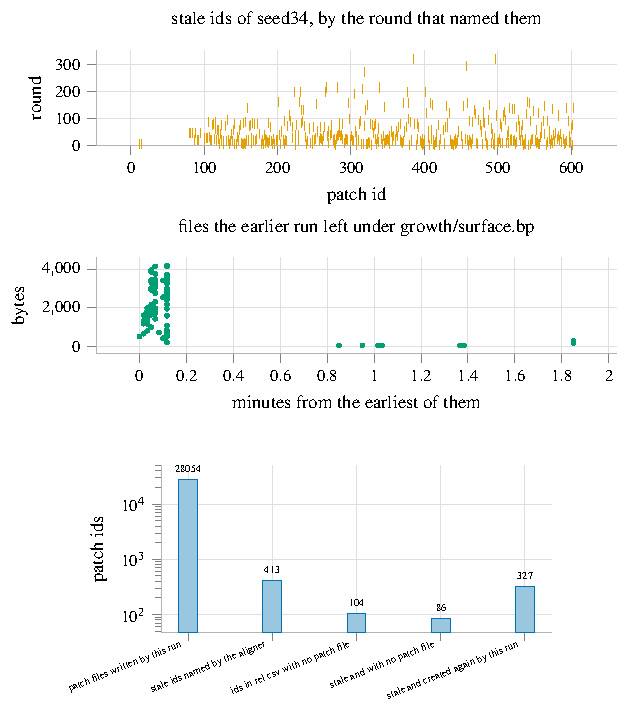
\includegraphics[width=\columnwidth]{figures/s-f4-seed34-two-runs-mixed}
\caption{\textbf{Two runs mixed in one folder.} A growth restarted into a folder that already held points does not start again, it adds. The run wrote \SeedPatchesThirtyFour{} patch files. The aligner's own log names \MixedImpossibleIds{} ids that cannot be this run's. \MixedOrphanIds{} ids appear in \protect\path{rel.csv} with no patch file at all, and \MixedImpossibleNoFile{} of them are among those stale ids. The number that matters is the last: \MixedImpossibleWithFile{} of the stale ids were created again by the second run, so most of the stale ids are invisible in the file listing and show only in the log. The crash of section 5 comes from the ones that are visible.}
\label{fig:s4}
\end{figure}

\section{What this does not change}

This section states what the acceleration leaves exactly as it was: every property of the delivered surface, and with it the distance to a 20 mm square.

Nothing in this work moves a square, and the reason is section 4. Every output is byte for byte what it was, so every property of the delivered surface is what it was, and every defect the stage had, it still has. What changed is how long the chain takes to produce the same answer, and on one tree, whether it produces one at all.

The distance to a 20 mm square is unchanged, and it is the honest frame for the whole work. The largest square this chain delivers on PHerc. 1447 is \SeedSquareTwentySix{} mm, drawn on the material in Fig.~\ref{fig:s5} {\prov{54}}. It is taken over the nine seeds whose growth finished: the three on papyrus of section 2 and the six tangles that grew in air. The best published segment of that same scroll reaches \BestPublishedSquare{} mm (Fig.~\ref{fig:s6}) {\prov{55}}. The chain is 0.8018 mm below it. That gap is inside this project's own repeat spread of \RepeatSpreadSquare{} mm {\prov{83}}, so it decides nothing either way.

\begin{figure*}[t]
\centering
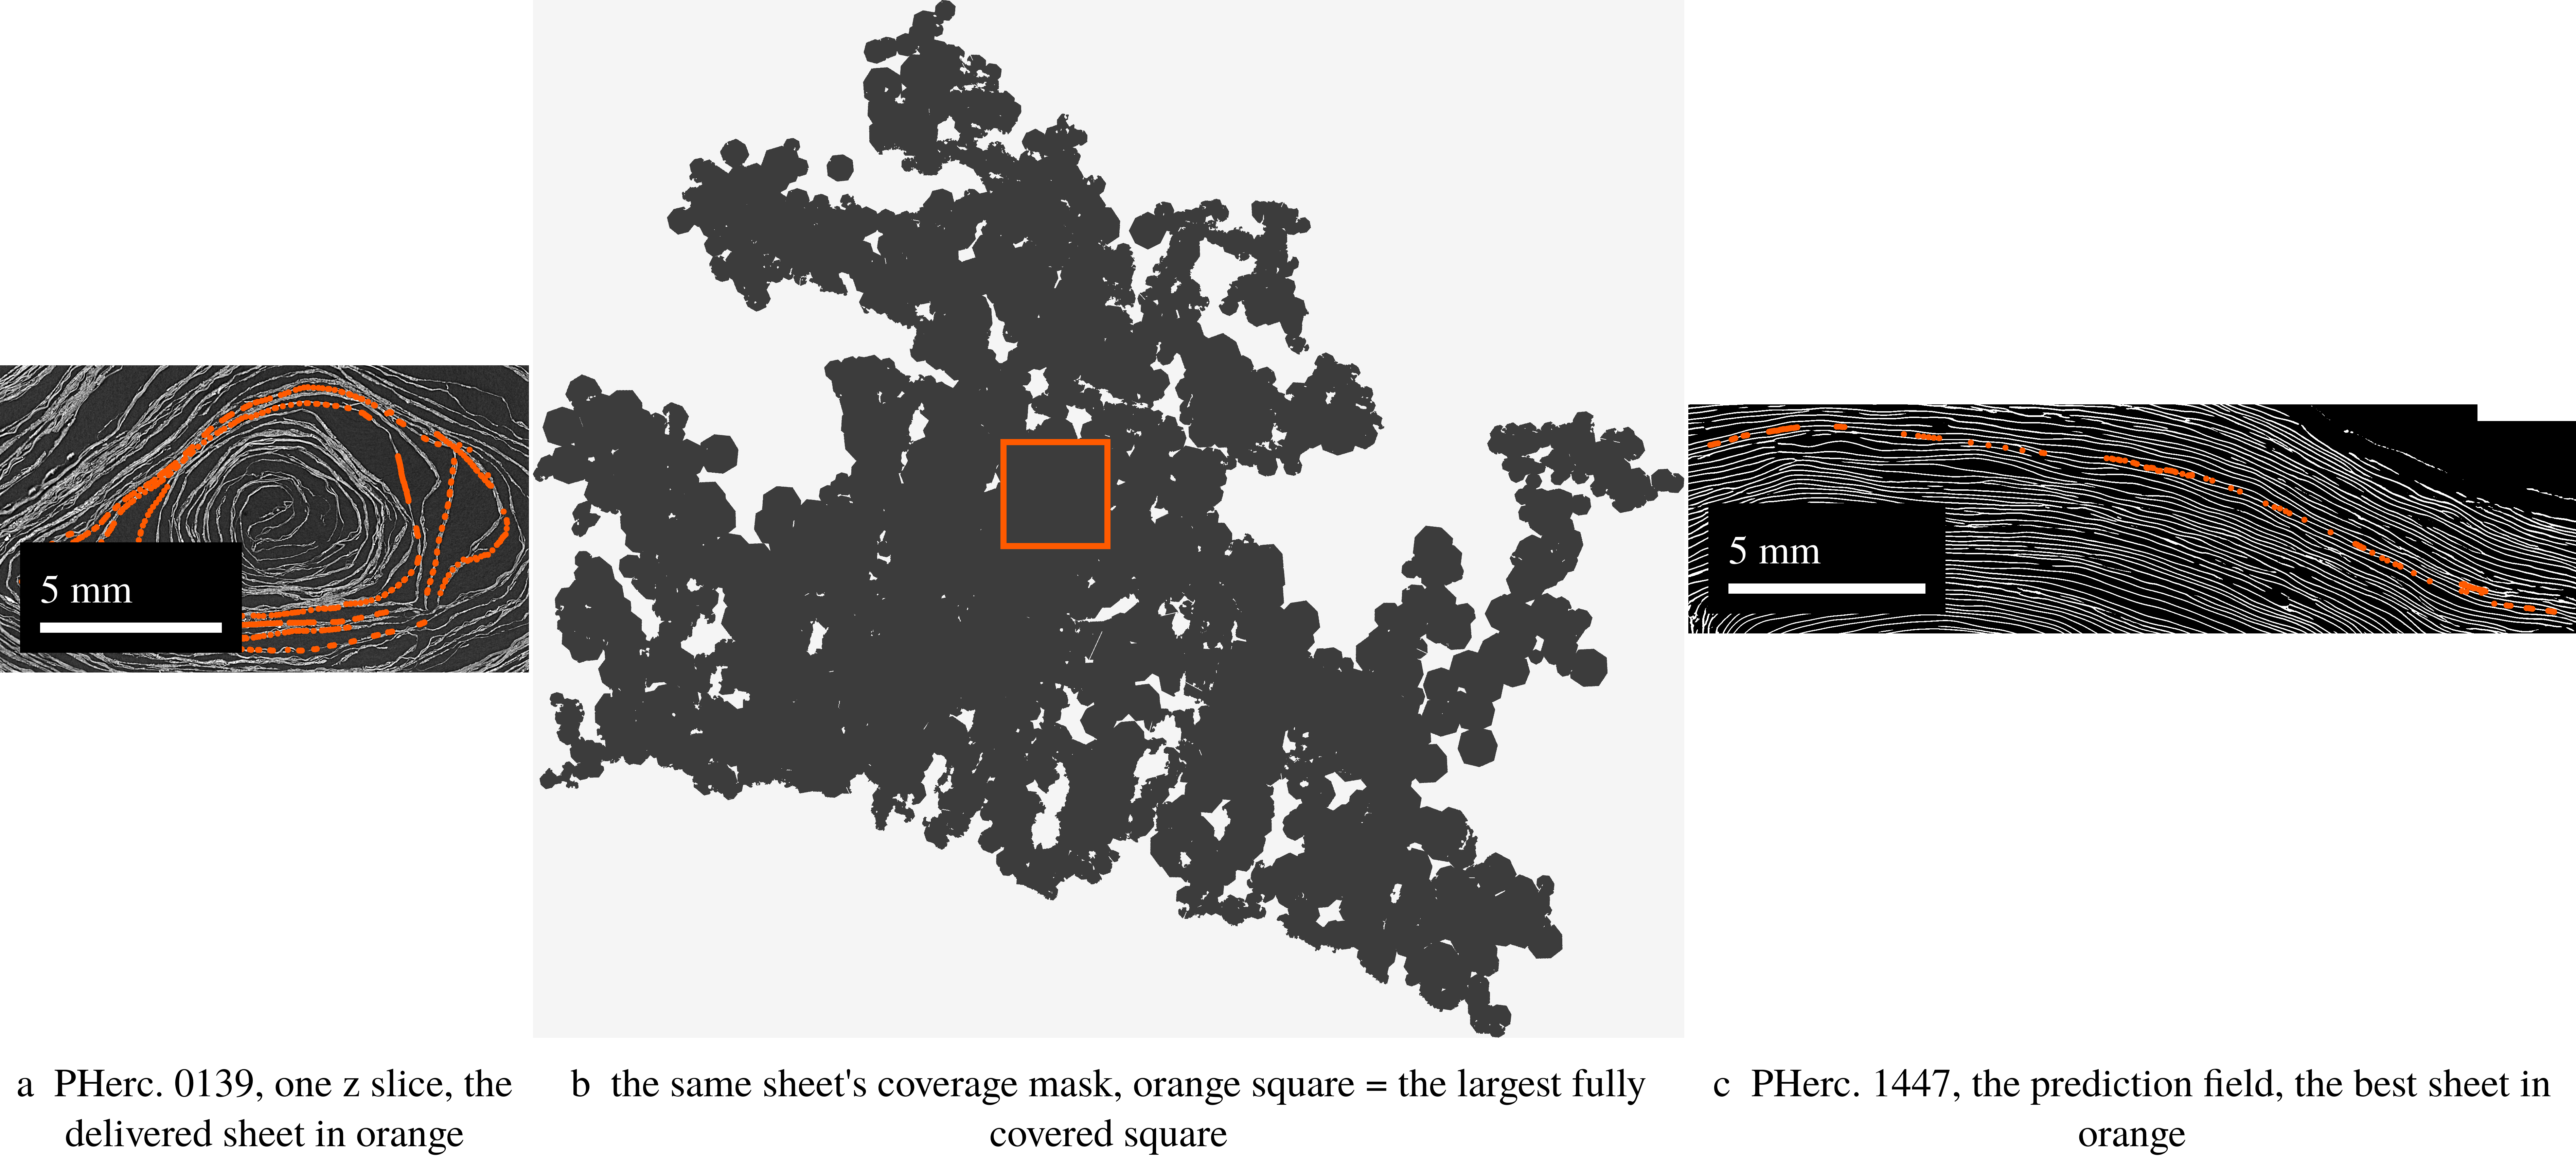
\includegraphics[width=\textwidth]{figures/s-f5-papyrus-with-the-sheet}
\caption{\textbf{Papyrus, with the delivered sheet on it.} The material, with the square the chain gets out of it. Panel a is one z slice of the reference scroll's own grayscale at full resolution, read from the raw scan, with 606 cells of a delivered sheet lying on it. Panel b is that sheet's coverage mask and the largest fully covered square in it, 324 cells on a lattice of \SheetLatticeI{} by \SheetLatticeJ{}. That square is \SheetSquareBase{} mm at \VoxelZeroOneThreeNine{} um a voxel, the largest over 610 measured sheets of twelve arms. Panel c is PHerc. 1447, whose grayscale is not on this disk, so the sheet is drawn on the published prediction field instead. The caption inside the figure says which of the two renderings each panel is. Its square is \SeedSquareTwentySix{} mm at 8.640 um a voxel. The two panels of papyrus are different renderings of different scrolls and are not to be compared pixel for pixel. What they share is the square. The white bars in panels a and c are 5 mm.}
\label{fig:s5}
\end{figure*}

\begin{figure}[t]
\centering
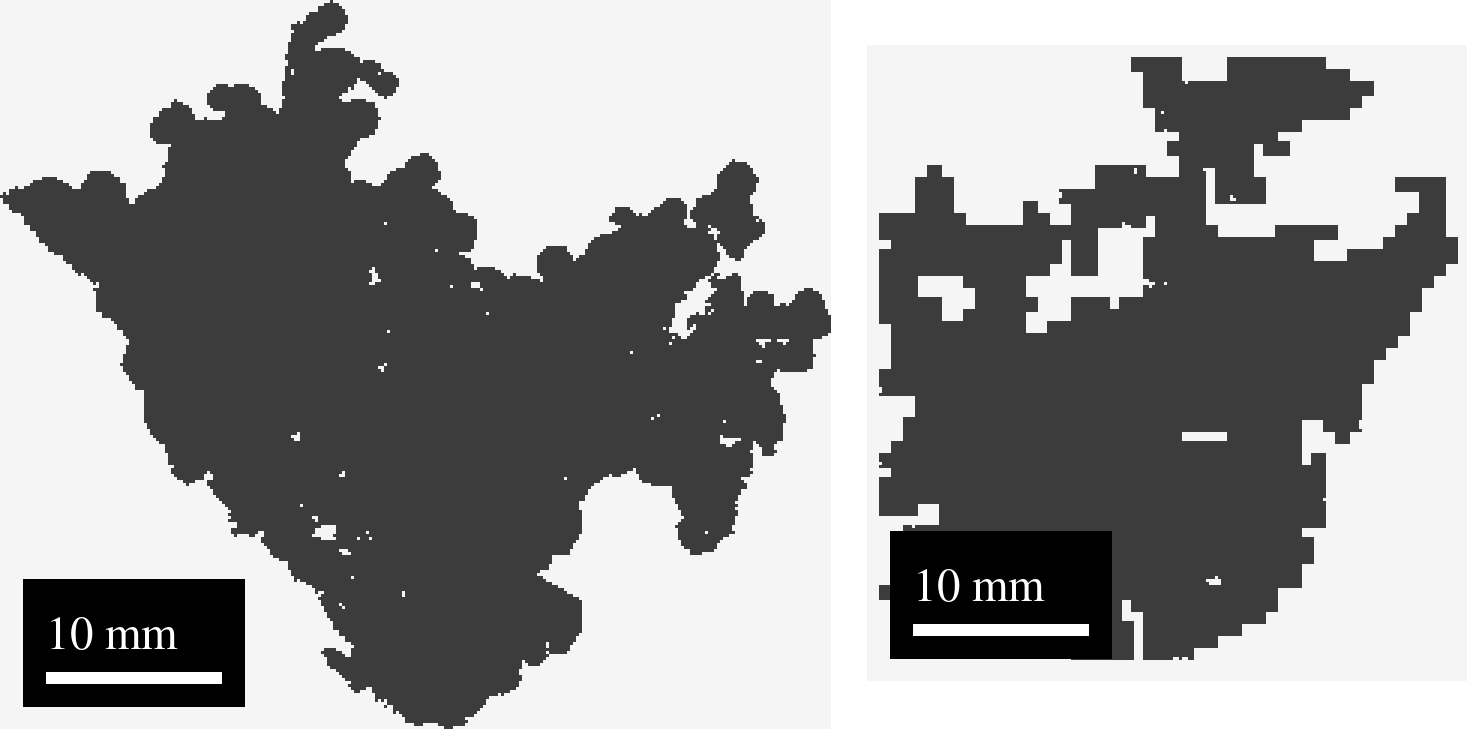
\includegraphics[width=\columnwidth]{figures/s-f6-coverage-beside-a-published-segment}
\caption{\textbf{Our coverage mask beside a published segment's, at the same scale.} Our best sheet of PHerc. 1447 reaches \SeedSquareTwentySix{} mm, recomputed over the 100 sheets that the ten seed files of the search measured. The best published segment of the same scroll reaches \BestPublishedSquare{}: the gap is 0.8018 mm, and this work claims nothing from it. The square is not drawn on the right panel, and the figure's own table says why in a row of its own. The segment's CSV measured a grid of 682 by 411 cells and the segment's tifxyz is 212 by 200, because the CSV read a different rendering of the same segment. A square placed on a grid it was not measured on would look like a measurement. Both panels are resampled to one millimetre per pixel, and the black bars are 10 mm.}
\label{fig:s6}
\end{figure}

The organisers' reference area is a contiguous 400 mm2, which is a 20 mm square, and the 20 mm side is the size the squares here are read against. None of the ninety sheets these nine seeds deliver reaches 20 mm {\prov{56}}. Nor does any of the twenty one published segments of PHerc. 1447 and PHerc. 0800 measured here {\prov{57}}.

So the acceleration buys search, not surface. It makes it cheap to ask the question on many seeds and it makes one class of tree deliverable at all. It does not bring the answer nearer to 20 mm by a millimetre, and nothing in this work should be read as saying it does.

The author's remedy for patches that cannot sit together is also unchanged by this work, and it is only half on in the chain as we automated it. Of its three methods~\cite{stevensreport12}, the bad patch finder runs, while the bridges and the annealing are manual steps that our runner never took {\prov{63}}. Put back together, the bridges and the annealing change the delivered sheets on \RemedySeedsChanged{} of \RemedySeedsMeasured{} seeds {\prov{64}}. The annealing draws from the hardware random device, so two runs on one tree are two draws and not a repeat {\prov{65}}, and a seed for it is offered as a correction.

\section{Limits}

This section sets out what the evidence does not establish. One caveat bears on the factor on the ribbon. On seed26 the untouched binary read 39.0 to 39.8 s on a loaded afternoon and \BenchPlainSeedTwentySixMax{} s on a quiet night. The changed binary's median moved far less, from \SpreadBothMedian{} to \BenchBothSeedTwentySixMedian{} s, and the cause is not known.

The mitigation is the one the bench has. The two arms of a ratio are measured back to back, on the same machine in the same state, so a common cause cancels. What does not cancel is comparing a number taken on one day with a number taken on another. The factors of the quiet bench do not mix the two, and the ratios of the shared machine are named as such where they appear. Where a figure from the earlier shared machine is still given, the table it sits in says so on its own line.

Four further limits have nothing to do with time. The first is the number of ribbons. The kinds of section 2 are nine growth trees of one scroll from one binary route, and only three of them are ribbons. Every threshold, band and ordering that rests on the ribbon group therefore rests on three points.

The second is that nine seeds are not the distribution. The maximum of nine is not the maximum of the draw.

The third is that the guard repairs the consumer, not the producer. Section 5 says the fault is in the growth's bookkeeping. Whether the producer should be repaired instead is a decision with its own declaration, and this work does not take it.

The fourth is that identity is not correctness. Every output of the changed arm is byte for byte the output of the unchanged one, and that is the whole of the claim. Whether the stage's answer is right is a different question and is not touched here.

\section{Open questions}

This section names the questions the evidence above raises and does not answer, each with what would settle it.

Does the annealing make the sheets better or worse? Put back with the bridges, it changes the delivered sheets, but each run is a new draw (section 6). With a seed read from the environment the draws become repeatable, and the chain with and without the annealing becomes a comparison instead of a draw.

Does the split between ribbons and tangles hold beyond three ribbons? The kinds of section 2 rest on nine growth trees of one scroll, of which only three are ribbons, so every threshold, band and ordering drawn from the ribbon group rests on three points (section 7). More ribbon trees grown and measured in the same way would say whether the split and the cost of the \texttt{c} stage on ribbons stay where they are.

\section{Conclusion}

Two changes inside the bad patch finder, S1 and S2, make its \texttt{c} stage finish on the tangles of PHerc.~1447, where it used to be abandoned. On the quiet bench the stage on the tangle seed40 is about two hundred times faster. Every file the five delivery stages write is byte identical with and without the changes on fifteen named trees of two scrolls, and so is the stage's whole standard output on fourteen of them (section 4). The guard, S3, turns an abort into a result on the one tree whose alignment file names patches with no file. Its cost in time on ribbons is more than covered by the two changes (section 5).

For someone running the chain, this changes how long a seed takes and not what it delivers. A tangle now costs its growth and about a minute of \texttt{c} stage rather than hours, so a search over many seeds becomes affordable. The squares, the defects and the distance to a 20 mm square stay exactly as they were (section 6). The three changes are proposed upstream as one pull request, stacked on the earlier performance patch they need (section 1).
